
\includegraphics[height=1.25cm]{images/pictograms/replication}

\includegraphics[height=1.25cm]{images/pictograms/benchmark}

\includegraphics[height=1.25cm]{images/pictograms/FEM}

\begin{flushright} {\tiny {\color{gray} python\_codes/fieldstone\_53/text.tex}} \end{flushright}

\lstinputlisting[language=bash,basicstyle=\small]{python_codes/fieldstone_53/keywords.ascii}

\begin{center}
Code at \url{https://github.com/cedrict/fieldstone/tree/master/python_codes/fieldstone_53}
\end{center}

\par\noindent\rule{\textwidth}{0.4pt}

This simple benchmark provides challenging numerical experiments 
dealing with large viscosity variations within the simulation
domain. It appears in \textcite{gery10} (2010) and consists of a bulk of fluid 1 ($\rho_1,\eta_1$)
in which a block of fluid 2 $(\rho_2,\eta_2)$ falls under its own
weight. The domain is a square of size $L_x=L_y=512~\si{\km}$ and the
block is initially centred at point ($x=256~\si{\km}$, $y=384~\si{\km}$) with size
$L_b\times L_b = 128~\si{\km}\times 128~\si{\km}$:

\begin{center}
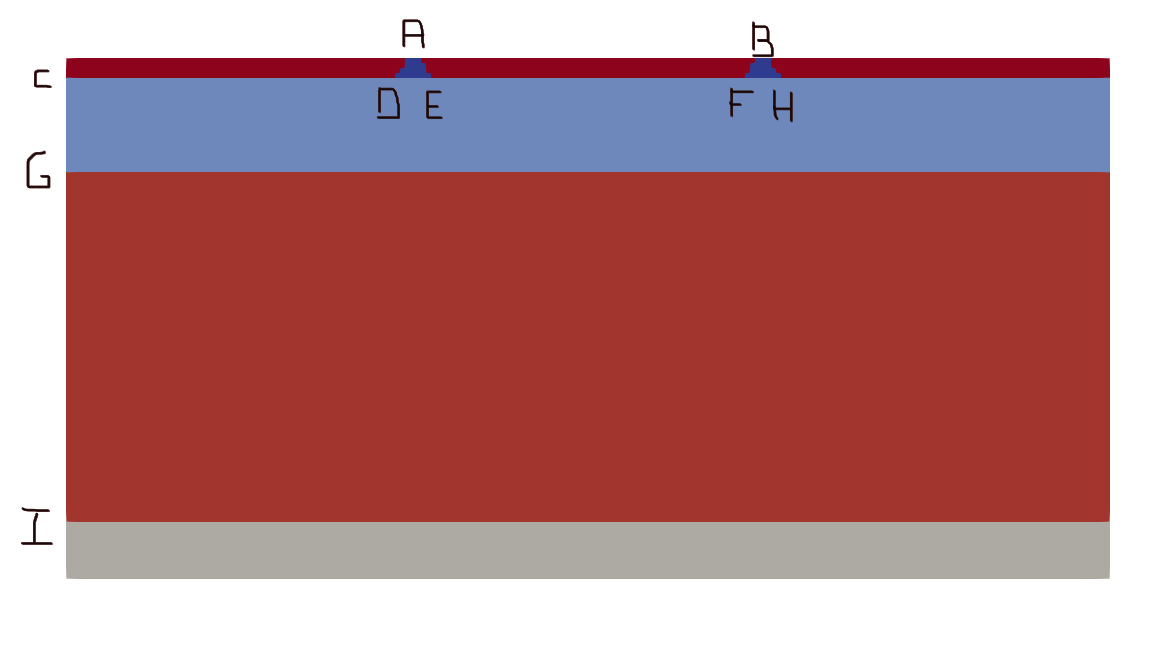
\includegraphics[height=6cm]{python_codes/fieldstone_53/images/setup}
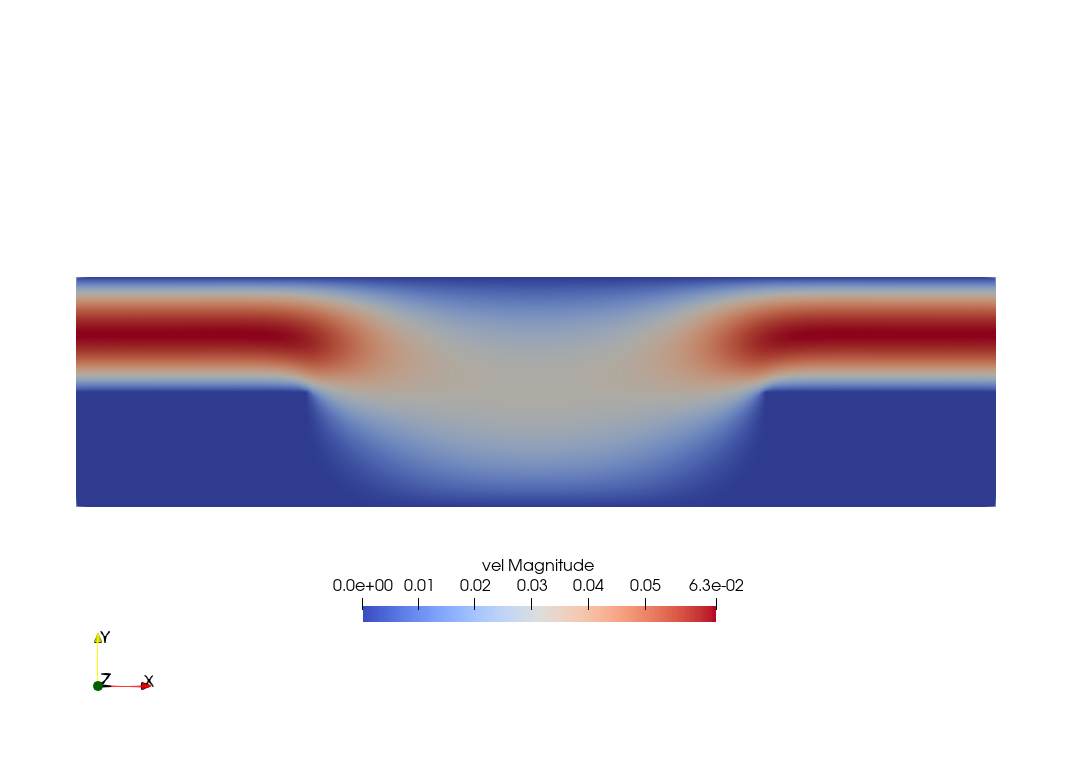
\includegraphics[height=6cm]{python_codes/fieldstone_53/images/vel}\\
{\captionfont Left: setup. Right: velocity field for $\rho_2=3208$, $\eta_1=10^{21}$
and $\eta_2=10^{22}$.}
\end{center}

The simulation is carried out on $32\times32$, $48\times48$ and $64\times 64$ grids. Free slip
boundary conditions are imposed on all sides of the domain. 
In all experiments the density of the surrounding fluid is $\rho_1=3200~\si{\kg\per\cubic\meter}$.
The velocity $v_b$ of the falling block is measured in its centre (note that due to symmetry 
the horizontal component should be zero).

As explained in \textcite{thie11} (2011), following physical intuition, one expects 
the velocity $v_b$ of the block to (a) decrease when the viscosity
of the surrounding medium $\eta_1$ increases; (b) increase with the
density contrast $\rho_2-\rho_1$. 
The quantity $v_b \eta_1/(\rho_2-\rho_1)$ is therefore monitored and shown hereunder as a function of 
the viscosity ratio.
We also then plot $p^\star=p/(\delta \rho g L_b)$ measured in the block center 
as function of $\eta_1/\eta_2$. 

%..........................
\paragraph{full density}

\begin{center}
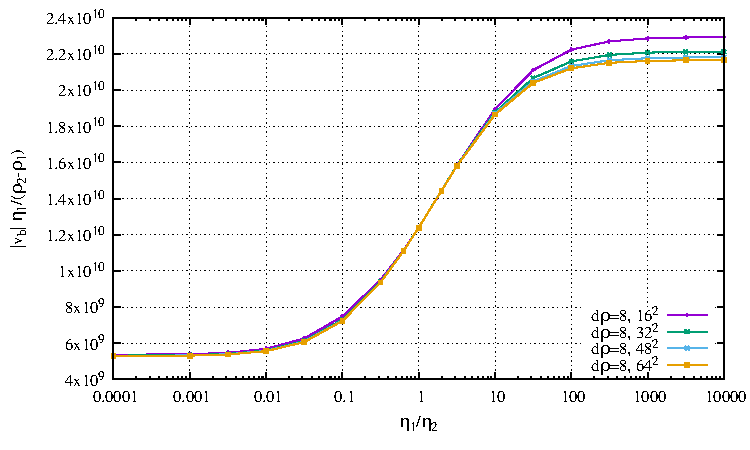
\includegraphics[width=8cm]{python_codes/fieldstone_53/results/full/results_v.pdf}
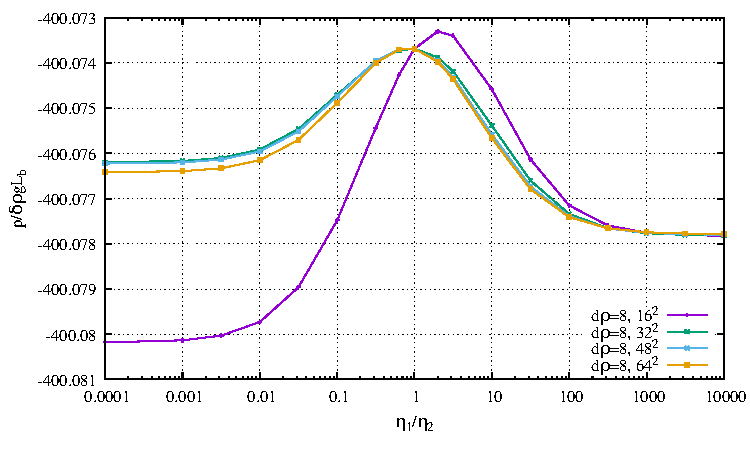
\includegraphics[width=8cm]{python_codes/fieldstone_53/results/full/results_p.pdf}\\
{\captionfont
Series of experiments have been conducted with $\rho_2=3208,3216$, 
$\log_{10}(\eta_1)=21$ and $\log_{10}(\eta_2)=17,18,...23,23.5,24,25$, 
all with 4 mesh resolutions.}
 \end{center}

All experimental points line up on a single curve which further
indicates that the code can deal with gravity driven simulations in the presence
of large viscosity contrasts. These results have been succesfully compared with 
those obtained with ASPECT with the same setup.

%..........................
\paragraph{reduced density}

Following the approach in \textcite{thba22} (2022), 
we set $\rho_1=0$ and $\rho_2=8$ so that we are only solving for the dydnamic 
pressure, the lithostatic pressure having been removed.

\begin{center}
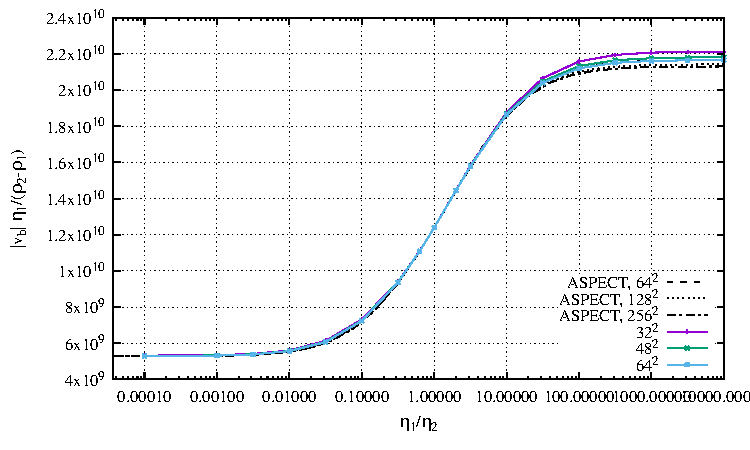
\includegraphics[width=8cm]{python_codes/fieldstone_53/results/reduced/results_v.pdf}
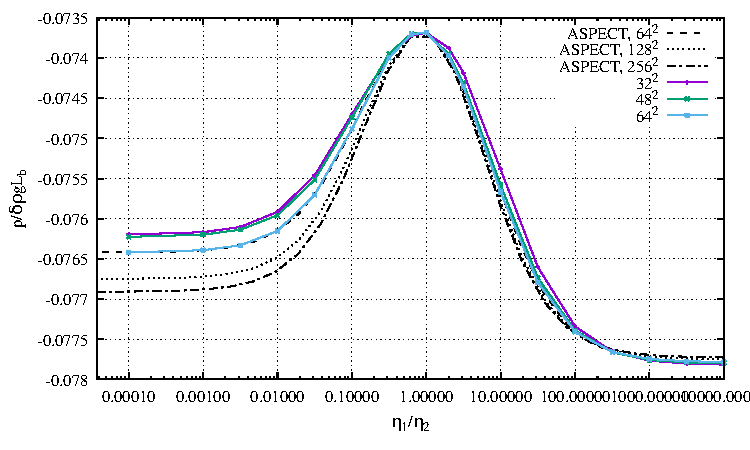
\includegraphics[width=8cm]{python_codes/fieldstone_53/results/reduced/results_p.pdf}\\
{\captionfont
Series of experiments have been conducted with $\rho_2=8$, 
$\log_{10}(\eta_1)=21$ and $\log_{10}(\eta_2)=17,17.5,18,..22.5,23,23.5,24$, 
all with multiple mesh resolutions.}
 \end{center}

We see that resolution $64\times 64$ is close but not quite {\sl the} solution of this experiment.

The pressure along the line $x=L_x/2$ was measured for 4 resolutions and both elements:
 
\begin{center}
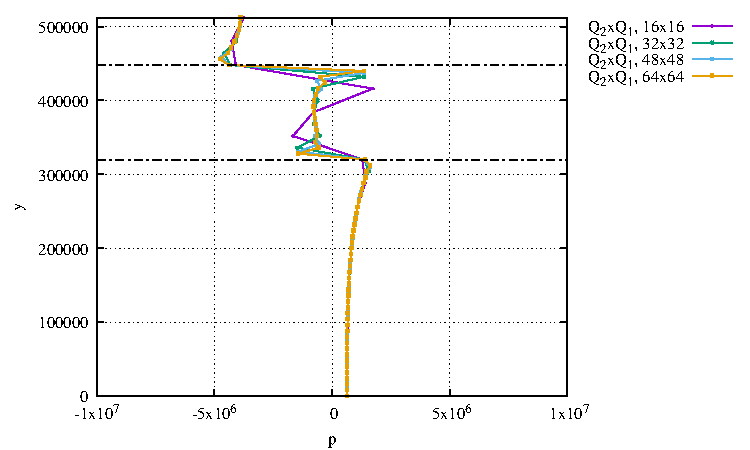
\includegraphics[width=8.3cm]{python_codes/fieldstone_53/results/reduced/plines_q2q1.pdf}
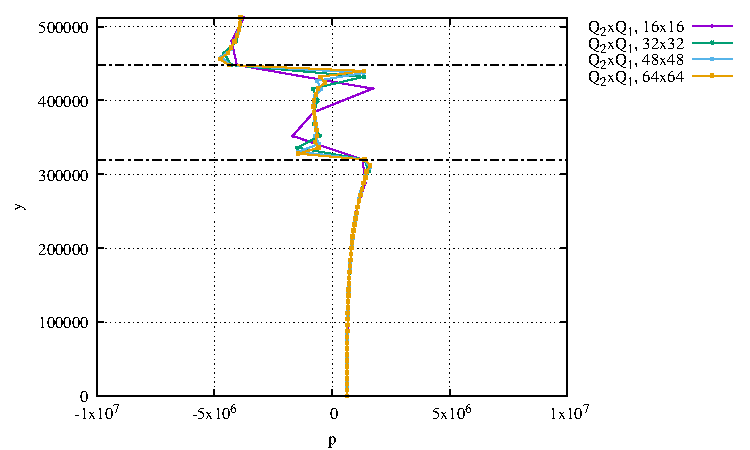
\includegraphics[width=8.3cm]{python_codes/fieldstone_53/results/reduced/plines_ser.pdf}\\
{\captionfont Left: $Q_2\times Q_1$ element; Right: $Q_2^{(8)}\times Q_1$ element.}  
\end{center}

